\documentclass[11pt]{amsart}
\usepackage{fancyhdr,graphicx,wrapfig,amsmath,amsthm,amssymb,latexsym}%,wrapfig,floatflt}
%\usepackage[matrix,arrow,cmtip,curve,dvips]{xy}
\DeclareGraphicsExtensions{.png}
\DeclareMathOperator{\im}{im}
\newcommand{\id}[1][{}]{\mathrm{Id}_{#1}}
\newcommand{\Q}{\mathbf Q}      % adds blackboard bold macros for
\newcommand{\R}{\mathbf R}      % conventional notation for
\newcommand{\Z}{\mathbf Z}      % rationals, reals, integers,
\newcommand{\C}{\mathbf C}      % complexes, naturals, field of p
\newcommand{\N}{\mathbf N}      % elements, p-adic integers
\newcommand{\D}{\mathbf D}
\newcommand{\Zp}{\mathbb{Z}_p}      % and numbers.
\newcommand{\Qp}{\mathbb{Q}_p}
\newcommand{\Fp}{\mathbb{F}_p}
\newcommand{\ie}{\emph{i.e.}}
\newcommand{\eg}{\emph{e.g.}}
\newcommand{\ind}[2]{[#1:#2]}       % index of groups, degree of field
\newcommand{\aut}[2][{}]{\mathrm{Aut}_{#1}(#2)}  % automorphism group
\newcommand{\isom}{\cong}       % isomorphic
\newcommand{\fk}[1]{\mathfrak{#1}}  % fraktur shorthand
\newcommand{\abs}[2][{}]{|#2|_{#1}} % generalized absolute value
\newcommand{\ord}[2][{}]{v_{#1}(#2)}    % roman ord(x), ord_p(x)
\newcommand{\Ex}{\begin{ex}}
\newcommand{\Eex}{\end{ex}}
\newcommand{\tr}[1]{#1^t}
\newcommand{\mat}[2]{M_{#1}(#2)}
\newcommand{\GL}[2]{\mathrm{GL}_{#1}(#2)}
\newcommand{\Lie}[1]{\mathrm{Lie}(#1)}
\newcommand{\ddt}[1]{\left. \frac{\mathrm{d}}{\mathrm{d}t} \right|_{t=#1}}
\newcommand{\ten}{\otimes}
\newcommand{\mg}[1]{{#1}^{\times}}
\newcommand{\wt}[1]{\widetilde{#1}}
\newcommand{\Tor}[2]{\mathrm{Tor}^{#1}_{#2}}

\theoremstyle{plain}            % define numbered and naked theorem
\newtheorem{ntheorem}{Theorem}[section]     % environments, numbered
\newtheorem{nlemma}[ntheorem]{Lemma}        % consecutively within
\newtheorem{nprop}[ntheorem]{Proposition}   % chapters
\newtheorem{ncor}[ntheorem]{Corollary}
\newtheorem*{theorem}{Theorem}
\newtheorem*{lemma}{Lemma}
\newtheorem*{prop}{Proposition}
\newtheorem*{cor}{Corollary}

% \newcounter{ntheorem}

\theoremstyle{definition}
\newtheorem{ndefn}[ntheorem]{Definition}
\newtheorem{nex}[ntheorem]{Example}
\newtheorem*{defn}{Definition}
\newtheorem*{ex}{Example}

%\theoremstyle{remark}
\newtheorem*{rmk}{Remark}
\newtheorem*{ntn}{Notation}

\usepackage{tabularx,dcolumn}
\usepackage[utf8]{inputenc}%
\usepackage[T1]{fontenc}%
\usepackage[fulloldstylenums,largesmallcaps]{kpfonts}%
\usepackage[english]{babel}
\usepackage[left=1in,right=1in,bottom=1in,top=1in]{geometry}
\usepackage{hyperref}

\setlength{\parskip}{1.0ex} \setlength{\parindent}{0pt}
\setlength{\headheight}{13pt} \setlength{\headsep}{8pt}

\pagestyle{fancy}
\linespread{1.01}
\lhead{Mathematics 431}
\chead{Spring 2013}
\rhead{February 11}
\lfoot{} \cfoot{} \rfoot{}

%\newcommand{\officehours}{TBA}
%\newcommand{\officehours}{T~10--12; W~2--3; F~1--2}

\begin{document}

\section{Introduction to Parametric Equations}

Let's begin by revisiting the idea of a \emph{function}. When most people think of a function, they are thinking of either a picture of the function (its \emph{graph}) or a table of its values. Let's give some names to the parties involved: the function is called $f$, its input variable or \emph{argument} is $x$, and its output variable or \emph{value} is $y$. In other words, $y = f(x)$. This gives us a third thing to imagine: the formula $f(x)$ by which the function $f$ is defined. (Is the function the same thing as the formula?)

This formula can be used, of course, to generate the ``table of values'', which I'll call a \emph{lookup table}, as well as the graph of $f$ in the usual way. One obtains for each value of $x$ along the horizontal axis in the $(x,y)$-plane a value of $y$ obtained by ``plugging in'' the particular values of $x$ into the formula. One then plots the points so obtained. For example, if $f(x) = x^2 - 3x + 2$, part of the table and graph are as follows.

\begin{figure}[ht]
\begin{minipage}[b]{0.45\linewidth}
%\begin{table}[h]
\begin{center}
\begin{tabular}{|c|c|}
\hline
$x$& $f(x)$  \\ \hline
$-2$ & $12$      \\ \hline
$-1$ & $6$  \\ \hline
$-0$ & $2$  \\ \hline
$1$  & $0$  \\ \hline
$2$  & $0$  \\ \hline
\end{tabular}
\end{center}
%\end{table}
\end{minipage}
\hspace{0.5cm}
\begin{minipage}[b]{0.45\linewidth}
\begin{center}
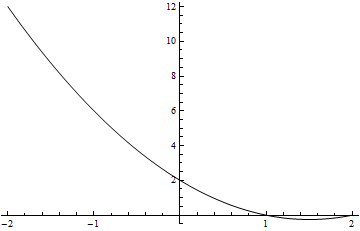
\includegraphics[width=\textwidth]{ch11se01-fig1}
\end{center}
\end{minipage}
\end{figure}
\begin{discussionquestion}
Why is each of these only a partial representation of the function? You should agree with your group members about a separate answer to this question for both the table and the graph.
\end{discussionquestion}

Most of the functions that we deal with can accept ``a lot'' of different numbers $x$ as their arguments---usually, an \emph{interval's worth} of numbers, or maybe a \emph{union of intervals' worth}. Remember that when we say ``interval'', we mean a set that might be infinite in the negative direction, the positive direction, or both.
\begin{example}
	The function $g_1$ defined by the formula $g_1(x) = x^2 - 3x + 2$ can accept any real number $x$ as its argument. Roughly, this is because the right-hand side of the defining equation for $g_1$ ``makes sense'' no matter which value of $x$ we might use. Mathematicians say $g_1$ is defined for all real numbers, or defined on the interval $(-\infty,\infty)$.
\end{example}
\begin{example}
	The function $g_2(x) = \sqrt{x}$ is defined on the interval $[0,\infty)$. This is the content of the familiar idea that only nonnegative numbers have square roots. (In the complex number system, things are different; we confine our discussion to real-valued functions of real variables.) Again, when we talk about the interval of definition of a function, we are talking about the admissible $x$-values. The collection of $y$-values that are thus produced is something else, which we'll discuss later.
\end{example}
\begin{discussionquestion}
	On which interval is the function $g_3(x) = \sqrt{1-x^2}$ defined? Justify your answer. (This phrase is one you will frequently encounter. It means that you should agree with your group members on a short paragraph that you all think is a convincing reason why your answer to the question is correct.)
\end{discussionquestion}
\begin{discussionquestion}
	For which values of $x$ is the function $g_4(x) = \tan(x)$ defined? Recall that $\tan(x) = \sin(x)/\cos(x)$ by definition. Express your answer as a union of intervals.
\end{discussionquestion}

If asked ``What is a function?'' by a very young person, or someone else with little experience of mathematics, we are tempted to identify the concept of the function with one of the three: its formula, its lookup table, or its graph. Many people, including many mathematicians, are intimidated by formulas, especially complicated ones. So with an amateur, we might be more inclined to use the lookup table or the graph to explain what functions are. We often use these ourselves, after all. But it's important to remember that they are only partial representations of a function. Somehow, the formula is more \emph{complete} than either the graph or the lookup table.

It is easy to make up a table (respectively, draw a curve in the $(x,y)$-plane) that is not the lookup table (respectively, graph) of any function. Remember the vertical line test? It's a property of curves in the plane.
\begin{discussionquestion}
	What is the vertical line test? How can you tell whether a curve passes it?
\end{discussionquestion}
A curve in the plane that fails the vertical line test isn't the graph of any function.
\begin{discussionquestion}
	Formulate a property of lookup tables that corresponds to the vertical line test for graphs.
\end{discussionquestion}
Functions often arise in physical contexts. We might view the height of a thrown ball as a function of time. This amounts to measuring the height at different moments and recording the times $t$ and the heights $s(t)$ as the arguments and values in a lookup table. Let's agree that the ball is thrown from height $0$ at time $0$. This is called ``choosing coordinates''. We don't have to worry about units if we don't want to. If you like you can impose some. Galileo realized that if the ball is thrown straight up with initial speed $v_0 > 0$, then the ball's height above its initial height at time $t$ is given by $s(t) = -at^2 + v_0 t$, where $a > 0$ is a constant that depends on the units of measurement. Here on the surface of Earth, we have $a \approx 9.8$ if we measure distance in meters and time in seconds.
\begin{discussionquestion}
 	What are appropriate units for the constant $a$ if we measure distance in meters and time in seconds? For the constant $v_0$?
\end{discussionquestion}
Why do we know that the height of a thrown ball satisfies the vertical line test? It has something to do with the causal structure of the world. The ball can only have one height at a time. It can be at the same height at many different times, but not have various heights all at the same time.

Now consider a bug crawling on a piece of paper, which is conveniently labeled with $x$- and $y$-axes. Its coordinates are completely independent of each other. Imagine that the bug leaves a visible trail on the page as we let it crawl around. If we let the bug crawl around long enough, the ``track'' or ``path'' it leaves will probably end up failing the vertical line test. All it has to do is move vertically or change horizontal direction, even for a moment. Unless it is always moving rightward (or always moving leftward), its track will fail the vertical line test and thus won't be the graph of any function. But we feel there must be formulas determining the position of the bug.

The key is to forget that we are so used to drawing functions' graphs in the $(x,y)$-plane and just think about a new kind of lookup table. I'll let the bug start crawling at $t = 0$ (again, seconds if you prefer), and record the $x$ and $y$ values every so often.

\begin{table}[h]
\centering
\begin{tabular}{|c|c|c|}
$t$ & $x(t)$ & $y(t)$ \\
0   & -1.00  & 2.00   \\
0.1 & -1.10  & 2.05   \\
0.2 & -1.00  & 2.10   \\
0.3 & -0.95  & 2.05   \\
\vdots & \vdots & \vdots
\end{tabular}
\end{table}


Here, it's important to remember that the lookup table omits lots of rows. We could have a more finely grained lookup table, with smaller steps in between adjacent $t$-values, or a more coarsely grained one, with larger steps. If I hand you a finely-grained lookup table like the one above, you can plot points along the corresponding bug path. For each row of the table, plot the point $(x(t),y(t))$, and connect the dots in order of increasing $t$-values.

This is called a parametric plot corresponding to the lookup table. Notice that the header row of the lookup table is very suggestive. It appears to imply that both the horizontal coordinate and the vertical coordinate are functions of the time variable $t$. Is this possible?
\begin{discussionquestion}
	If a bug walks around the $(x,y)$-plane in the manner described above, are its $x$- and $y$-coordinates functions of time $t$? (Remember, the answer to this question has something to do with the vertical line test and its lookup table analogue. We aren't saying anything about these functions' formulas yet.)
\end{discussionquestion}

Now let's generalize, coming to the definition of parametric equations. If we have two functions $f(t)$ and $g(t)$ that are defined for the same arguments (the same $t$ values), we can make a 3-column parametric lookup table as above, and hence we can plot a curve in the plane by following the moving point $(f(t), g(t))$. We say that $x = f(t)$ and $y = g(t)$ are \emph{parametric equations} for the curve thus generated.

We might just as well think of the \emph{point} $(f(t), g(t))$ as the value of a function (it's the location of the bug, just like earlier we let $s(t)$ be the height of the ball), rather than try to separate the coordinates into two functions. We can write
\[
	c(t) = (f(t), g(t))
\]
and think of $c$ as some kind of function. If this makes you a bit uncomfortable, good! Function are supposed to have \emph{numbers} as their values (outputs), but the right-hand side of the above equation is a point, not a number. This is OK, and we'll deal with the technical details later. For now, just know that a set of parametric equations $x = f(t)$, $y = g(t)$, is the same thing as a moving point $c(t) = (f(t),g(t))$: that is, a particle whose location depends on time.

The most important set of parametric equations in the world is:
\[
	x = \cos(t), \quad y = \sin(t).
\]
\begin{discussionquestion}
	Using a calculator, or better, using your knowledge of the behavior of the sine and cosine functions, determine which plane curve comes from these parametric equations.
\end{discussionquestion}
\begin{discussionquestion}
	Repeat the last question for the parametric equations
	\[
		x = \cos(-t), \quad y = \sin(-t).
	\]
\end{discussionquestion}

The second most important (maybe it's a tie) kind of parametric equation to recognize is \emph{parametrizations of lines}. Actually, we'll only worry about parametrizations of a certain form. These will turn out to be the parametrizations of constant speed, as we'll see soon. Let's develop these parametrizations in a different way than is done in the textbook.

Imagine a line in the plane---a non-vertical one for now. If asked to specify it algebraically (by means of an equation relating the coordinates of points belonging to it) most of us would choose to use the standard form
\[
	y = mx + b,
\]
in which $m$ by long tradition stands for the slope and $b$ for the $y$-intercept. One reason we are so inclined to prefer this form is because it displays $y$ as a function of $x$. (Of course, the vertical lines are ironically exactly the ones that fail the vertical line test and hence cannot be so written.) Let us think briefly about what $m$ and $b$ really mean. The line must pass through $(0,b)$: that is the significance of $b$. We'll call $(0,b)$ the \emph{starting point}. This is where our bug sits when $t = 0$. 

Now I will state a somewhat surprising fact: There is no ``natural'' choice of our bug's position at $t = 1$ (or at any other time). Nothing about the shape of the bug's path determines its velocity. This is a choice we have to make. Every choice of velocity gives a different parametrization of the line\footnote{The observant reader will note that the bug doesn't have to have a constant velocity, and hence there are even more parametrizations than we describe here}.

For concreteness, let $m = 2/3$ and $b = 2$. We may choose any other point on the line as the $t = 1$ position, say $(3,4)$. If the bug's velocity doesn't change, then by $t = 2$ it will have reached $(6,6)$. Extending its trajectory backward in time to $t = -1$ we find that the position should be $(-3,0)$. Since the bug travels
\[ 
 	\sqrt{(4-2)^2 + (3-0)^2} = \sqrt{4+9} = \sqrt{13}
\]
for each tick of the clock, we may say its speed is $\sqrt{13}$ (in this parametrization). (Notice I say speed and not \emph{velocity}; we'll return to this point later.)

Now there's nothing special about $\sqrt{13}$. We can give the bug any nonzero speed we like and have it travel along the line in either direction. All of these will yield parametrizations of the line. To get all of these algebraically at once, let's return to the situation above, where we've chosen $(0,2)$ as the starting point, but not yet chosen a $t = 1$ point. Now instead of choosing a second point on the line, let's just choose the ``run'' from $(0,2)$ to our second point. This is the horizontal distance. Call this run $r$. The second point, when $t = 1$, therefore has $x$-coordinate $0 + r = r$. The rise $s$ can be computed from the slope:
\[
	s = \frac{2}{3} r.
\]
The interpretation of $s$ is that $2 + s$ is the $y$-coordinate of the $t = 1$ point. Now where is the point at $t = 2$? Evidently its location is
\[
	((0+r)+r,(2+\frac{2}{3} r)+\frac{2}{3} r) = (0+2r,2+2\frac{2}{3} r) = (0+2r,2+\frac{4}{3} r,
\]
and more generally, at any time $t$, our point lives at
\[
	(0+rt,2+(\frac{2}{3}r)t).
\]
This is the vector form of all parametrizations (again, with constant speed) of the line through $(0,2)$ with slope $2/3$. The parametric form is
\[
	x = rt, \quad y = 2 + \frac{2r}{3}t.
\]
Since we can choose any nonzero value for $r$ (why do we need $r \ne 0$?) we see there are indeed infinitely many parametrizations of this sort, as claimed. Observe that $s/r = 2/3 = m$. Therefore we have confirmed the description given in the text. It's essential that you be able to parametrize lines in this way, and that you be able to recognize the above equations as the parametric equations of a line.

This example illustrates a key difference between graphs of ordinary functions and parametrized curves. If a curve $C$ is a graph, then there's only one function whose graph it is. But just like for straight lines, there are lots of ways to parametrize a given curve: infinitely many, in fact, because we can traverse the curve at any speed we like. 

\begin{discussionquestion}
	If you have a lookup table (either for an ordinary function or for a set of parametric equations) you can easily draw part of the corresponding curve. How can you go ``backwards'', that is, if you only have a picture of the curve, how can you construct the lookup table? Is your answer the same in the parametric and the nonparametric case?
\end{discussionquestion}

Suppose we are given a function $f(x)$. It is very easy to parametrize the graph of such a function: think of it in terms of lookup tables. The table on the left is the lookup table of the function $f(x)$ and the table on the right is a partial lookup table for a parametrization of the graph.
\begin{figure}[ht]
\begin{minipage}[b]{0.45\linewidth}
\centering
\begin{tabular}{c|c}
	$x$ & $y$ \\ \hline
	$x_0$ & $f(x_0)$ \\
	$x_1$ & $f(x_1)$ \\
	$x_2$ & $f(x_2)$ \\
	\vdots & \vdots
\end{tabular}
\end{minipage}
\hspace{0.5cm}
\begin{minipage}[b]{0.45\linewidth}
\centering
\begin{tabular}{c||c|c}
	$t$ & $x$  & $y$ \\ \hline
	  & $x_0$ & $f(x_0)$ \\
	  & $x_1$ & $f(x_1)$ \\
	  & $x_2$ & $f(x_2)$ \\
	\vdots & \vdots & \vdots
\end{tabular}
\end{minipage}
\end{figure}
Converting the functional description of a curve to a parametric description is the same as filling in the table on the right. But remember! most of the rows in the table aren't shown. This means that trying something like 0, 1, 2, \dots\ won't work. It doesn't say what happens for all the rows that don't appear in our table. So there's really only one idea that will work.

\begin{center}
\begin{tabular}{c||c|c}
	$t$ & $x$  & $y$ \\ \hline
	$x_0$ & $x_0$ & $f(x_0)$ \\
	$x_1$ & $x_1$ & $f(x_1)$ \\
	$x_2$ & $x_2$ & $f(x_2)$ \\
	\vdots & \vdots & \vdots
\end{tabular}
\end{center}

We can simply make the $t$-column the same as the $x$-column. In other words, we let $x = t$ for all $t$. Then the parametric and vector forms we obtain are
\[
	x = t, \quad y = f(t) \qquad \text{and} \qquad c(t) = (t, f(t)).
\]
If it bugs you that $y = f(t)$ now instead of $f(x)$, don't worry; after all, we insisted that $x = t$ for all $t$.

Converting a parametric or vector description of a curve to a functional description isn't so easy, usually. The book kind of gives you the wrong idea. The examples in which it's possible are really unusual. It's enough for me if you can recognize the circles and lines. 
\end{document} 